\section{Evaluation}
\label{sec:goal}
To evaluate the indirection technique, we implemented the formulations described
in Section~\ref{sec:noindirection} and ~\ref{sec:indirection} , and then used the Gurobi
ILP solver~\cite{gurobi}
to find the optimal solution. To get a nearly optimal solution within a reasonble time,
we used a callback function which will terminate the ILP solver if the optimality gap (MIPGap) is
less than 0.1\% and the current best solution didn't change for 5 minutes.

Although ILP solver gives optimal solution to the scheduling problem, it can't scale since there
are O($n!$) different configuratons to be considered for scheduling. To the end of this, we
propose a post-scheduling merging heuristic. Given a scheudule computed by a scheudling algorithm
(e.g. Solstice), this merging heuristic uses indirection technique to reduce the number
of distinct configurations needed, and thus reduce the total time to serve all demand.
We received the simulator of the Solstice algorithm from the authors, and introduced
our merging techinque into the simulator to compare it with the original Solstice algorithm.

We built 100 skewed matrices (12 hosts) as the input demand matrices. For each input demand
matrix, we use ILP solver (with and without indirection), Solstice algorithm, Solstice+Merging
to schedule the demand. Figure~\ref{fig:time} and ~\ref{fig:conf} depcit the results. Comparing
the ILP results, indirection technique reduces the average number of configurations from 8.12 to
4.35, which leads to a 3.125\% reduction on the total time. For the simulation results, the
merging heuristic helps the Solstice to reduce the average number of configurations from 14.40 to
10.63, which leads to a 2\% reduction on the total time. This shows that our merging hueristic
provides similar improvement on Solstice as the ILP results. We believe that the merging heuristic
could provide increasing improvement at a larger scale since Solstice will use even more configurations
to schedule the demand.

\begin{figure}[t]
    \center
    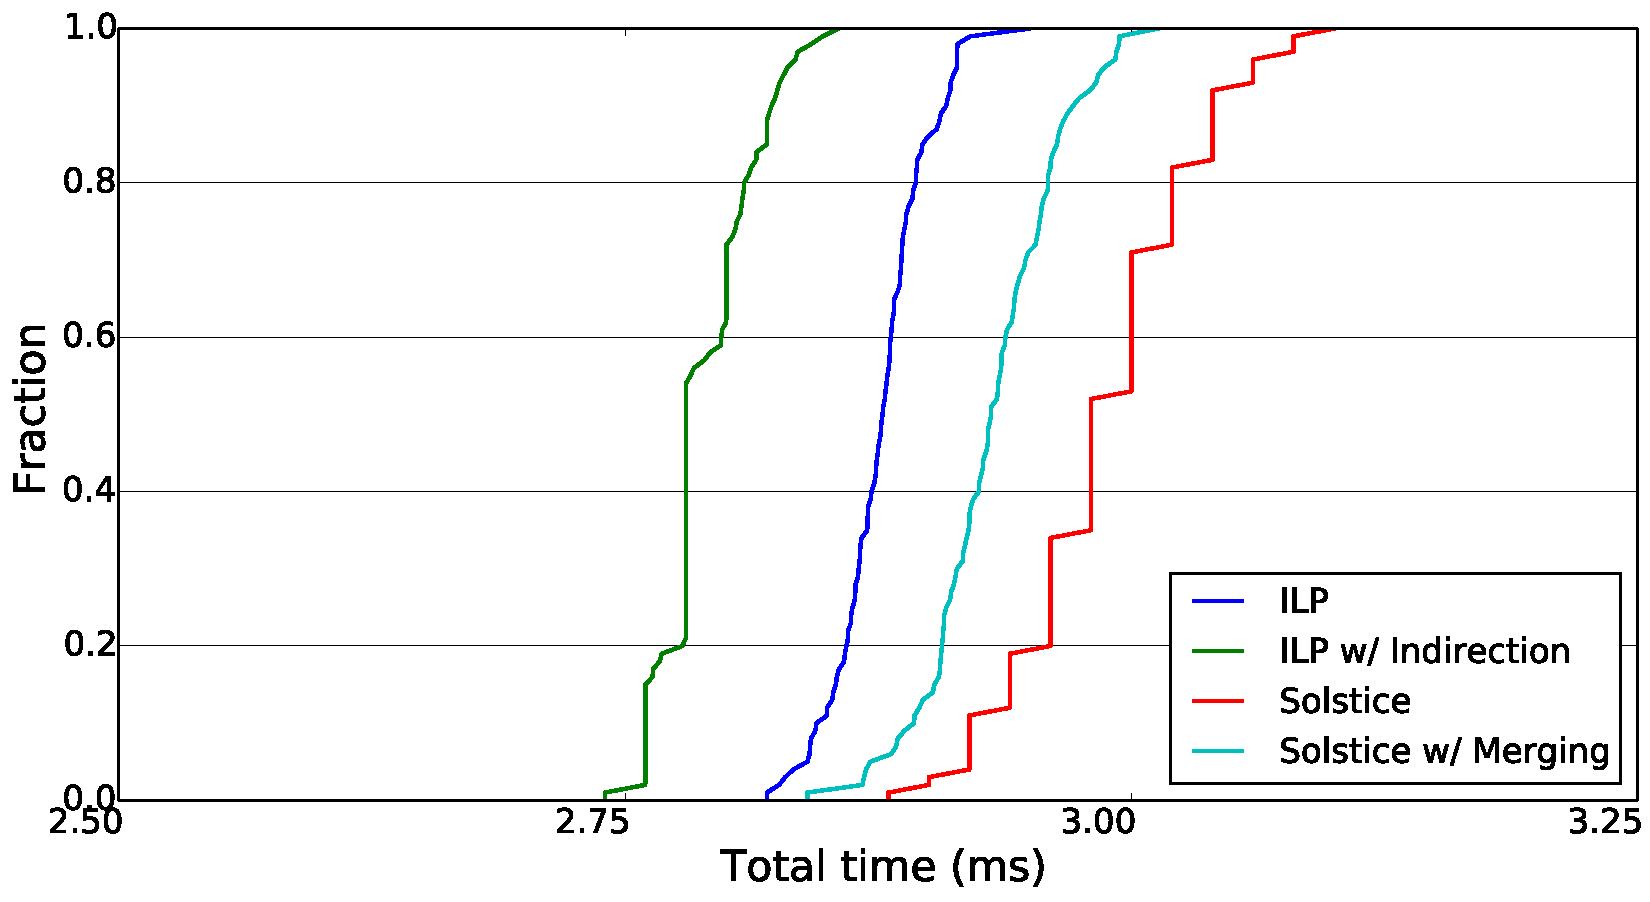
\includegraphics[width=5in]{time.pdf}
    \caption{\label{fig:time}CDF of total time required when serving 100\% demand. Average: 2.88, 2.79, 2.99, 2.93.}
\end{figure}

\begin{figure}[t]
    \center
    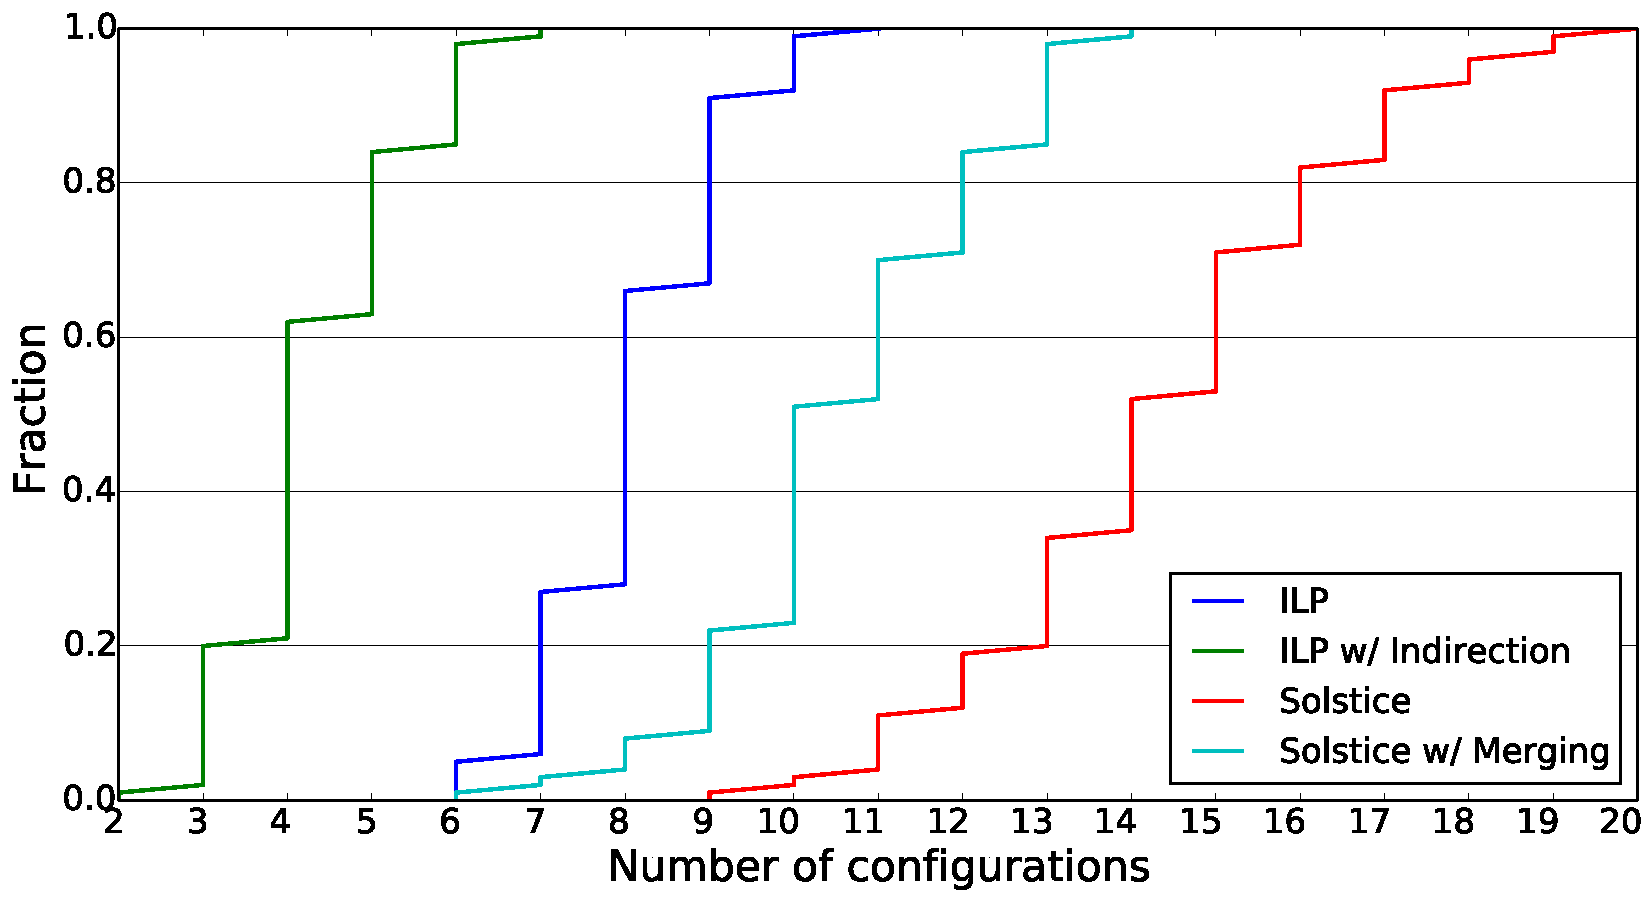
\includegraphics[width=5in]{conf.pdf}
    \caption{\label{fig:conf}CDF of number of configurations required when serving 100\% demand. Average: 8.12, 4.35, 14.40, 10.63.}
\end{figure}

\section{Conclusion}
\label{sec:conclu}

Recent advances in optical switch technology has created a need for new scheduling
algorithms which take advantage of shorter reconfiguration times while maintaining
reasonable computational overheads. The recent Solstice scheduling algorithm
accomplishes these goals, but does not achieve optimal utilization due to the
fact that it only supports traffic sent over a direct link.
It is possible to meet traffic demands without utilizing a direct link between
each source and destination port by routing traffic over multiple links.
Utilizing these indirect links can reduce the number of reconfigurations necessary
and reduce the amount of unused bandwidth on each link.

In this paper, we have presented an extension to the Solstice packet scheduler allowing for
multi-hop indirect serving of traffic. Through comparison with the original
algorithm in simulation, we have demonstrated that
this indirection technique reduces the number of reconfigurations necessary to serve
all traffic demand by increasing the utilization of each link. 
Our evaluation shows that the indirection technique does not have prohibitively high
computational overhead, and decreases the total amount of time necessary to fulfill
all traffic demands. 
